% !TEX program = xelatex
\documentclass[a4paper]{article}
\usepackage{amsthm}
\usepackage{amssymb}
\usepackage{bm}
\usepackage{mathtools}
\usepackage[x11names]{xcolor}
\usepackage{xparse}
\usepackage{fontspec}
\usepackage{unicode-math}
\setromanfont{DovesType-Regular.otf}
\setsansfont{Andika}
\setmathfont{Asana Math}[Scale=1]
\newfontfamily\TrajanP[Scale=1.0]{TRAJANPRO-REGULAR.OTF}
% \newfontfamily\TrajanP[Scale=1.0]{Tork}

% \usepackage{pstricks}
\usepackage{varwidth}
\usepackage{siunitx}
\usepackage{graphicx}
\usepackage[margin=1.5cm,top=1.5cm]{geometry}
\usepackage[most]{tcolorbox}
\usepackage{pgfplots}
\pgfplotsset{compat=newest}
\tcbuselibrary{skins,xparse,poster,breakable}
% \usetikzlibrary{fadings}
\usetikzlibrary{calc,math, plotmarks, shapes, shapes.geometric, positioning, angles, intersections, quotes, through, patterns, turtle, arrows.meta}
\usetikzlibrary{decorations.markings,backgrounds}
% \usepackage{etoolbox}
\usepackage{tkz-euclide}
% \usepackage{xlop}
% \newcommand\hole[2]{#1}  % for use with xlop
\pagenumbering{gobble}
%%%%%%%%%%%%%%%%%%%%%%%%%%%%%%%%%%%%%%%%%%%%%%%%%%%%%%%%%
\newcommand\markangle[9]{% origin X Y radius radiusmark mark colour opacity
%  % fill red circle offset-from-centre
  \begin{scope}
    \path[clip] (#1) -- (#2) -- (#3);
    \fill[color=#7,fill opacity=#8,draw=black,name path global=pcircle]  % global declaration required otherwise pcircle is not seen by the `named intersections=' lines below.
    (#1) circle (#4);
  \end{scope}
  % middle calculation
  \path[name path=line one] (#1) -- (#2);
  \path[name path=line two] (#1) -- (#3);
  \path[%
  name intersections={of=line one and pcircle, by={inter one}},
  name intersections={of=line two and pcircle, by={inter two}}
  ] (inter one) -- (inter two) coordinate[pos=#9] (place);
  % put mark
  \node at ($(#1)!#5!(place)$) {\scriptsize{#6}};
}

\newcommand\tcircle[6]{% centre coord (x,y), radius, points, radpoint, colour, edge
  \coordinate (O) at (#1,#2); % centre of the circle
  \def\radius{#3}          % radius of the circle
  \def\npts{#4}            % number of the points
  \def\radpt{#5}           % radius of the points
  \colorlet{ptcolour}{#6}  % colour of the points
  % \draw (O) circle (\radius);
  \foreach \numpoint in {1,...,\npts}{
    \fill[ptcolour] (O) ++ (360/\npts*\numpoint:\radius) coordinate (C\numpoint) circle(\radpt);
  }
}

% \newcommand{\condSoln}[2]{\ifcsdef{r@#1}{#2}{}}

% \newcommand\fadingtext[3][]{%
%    \begin{tikzfadingfrompicture}[name=fading letter]
%      \node[text=transparent!0,inner xsep=0pt,outer xsep=0pt,#1] {#3};
%    \end{tikzfadingfrompicture}%
%    \begin{tikzpicture}[baseline=(textnode.base)]
%      \node[inner sep=0pt,outer sep=0pt,#1](textnode){\phantom{#3}};
%      \shade[path fading=fading letter,#2,fit fading=false]
%      (textnode.south west) rectangle (textnode.north east);%
%    \end{tikzpicture}%
% }

\definecolor{JISpurple}{RGB}{89,72,122}
\definecolor{JISivory}{RGB}{241,234,221}
\definecolor{JIStaupe}{RGB}{183,156,154}
\definecolor{PaleGreen}{RGB}{240,255,240} % 'Honeydew'

\AddToHook{shipout/background}{%
    \put (0in,-\paperheight){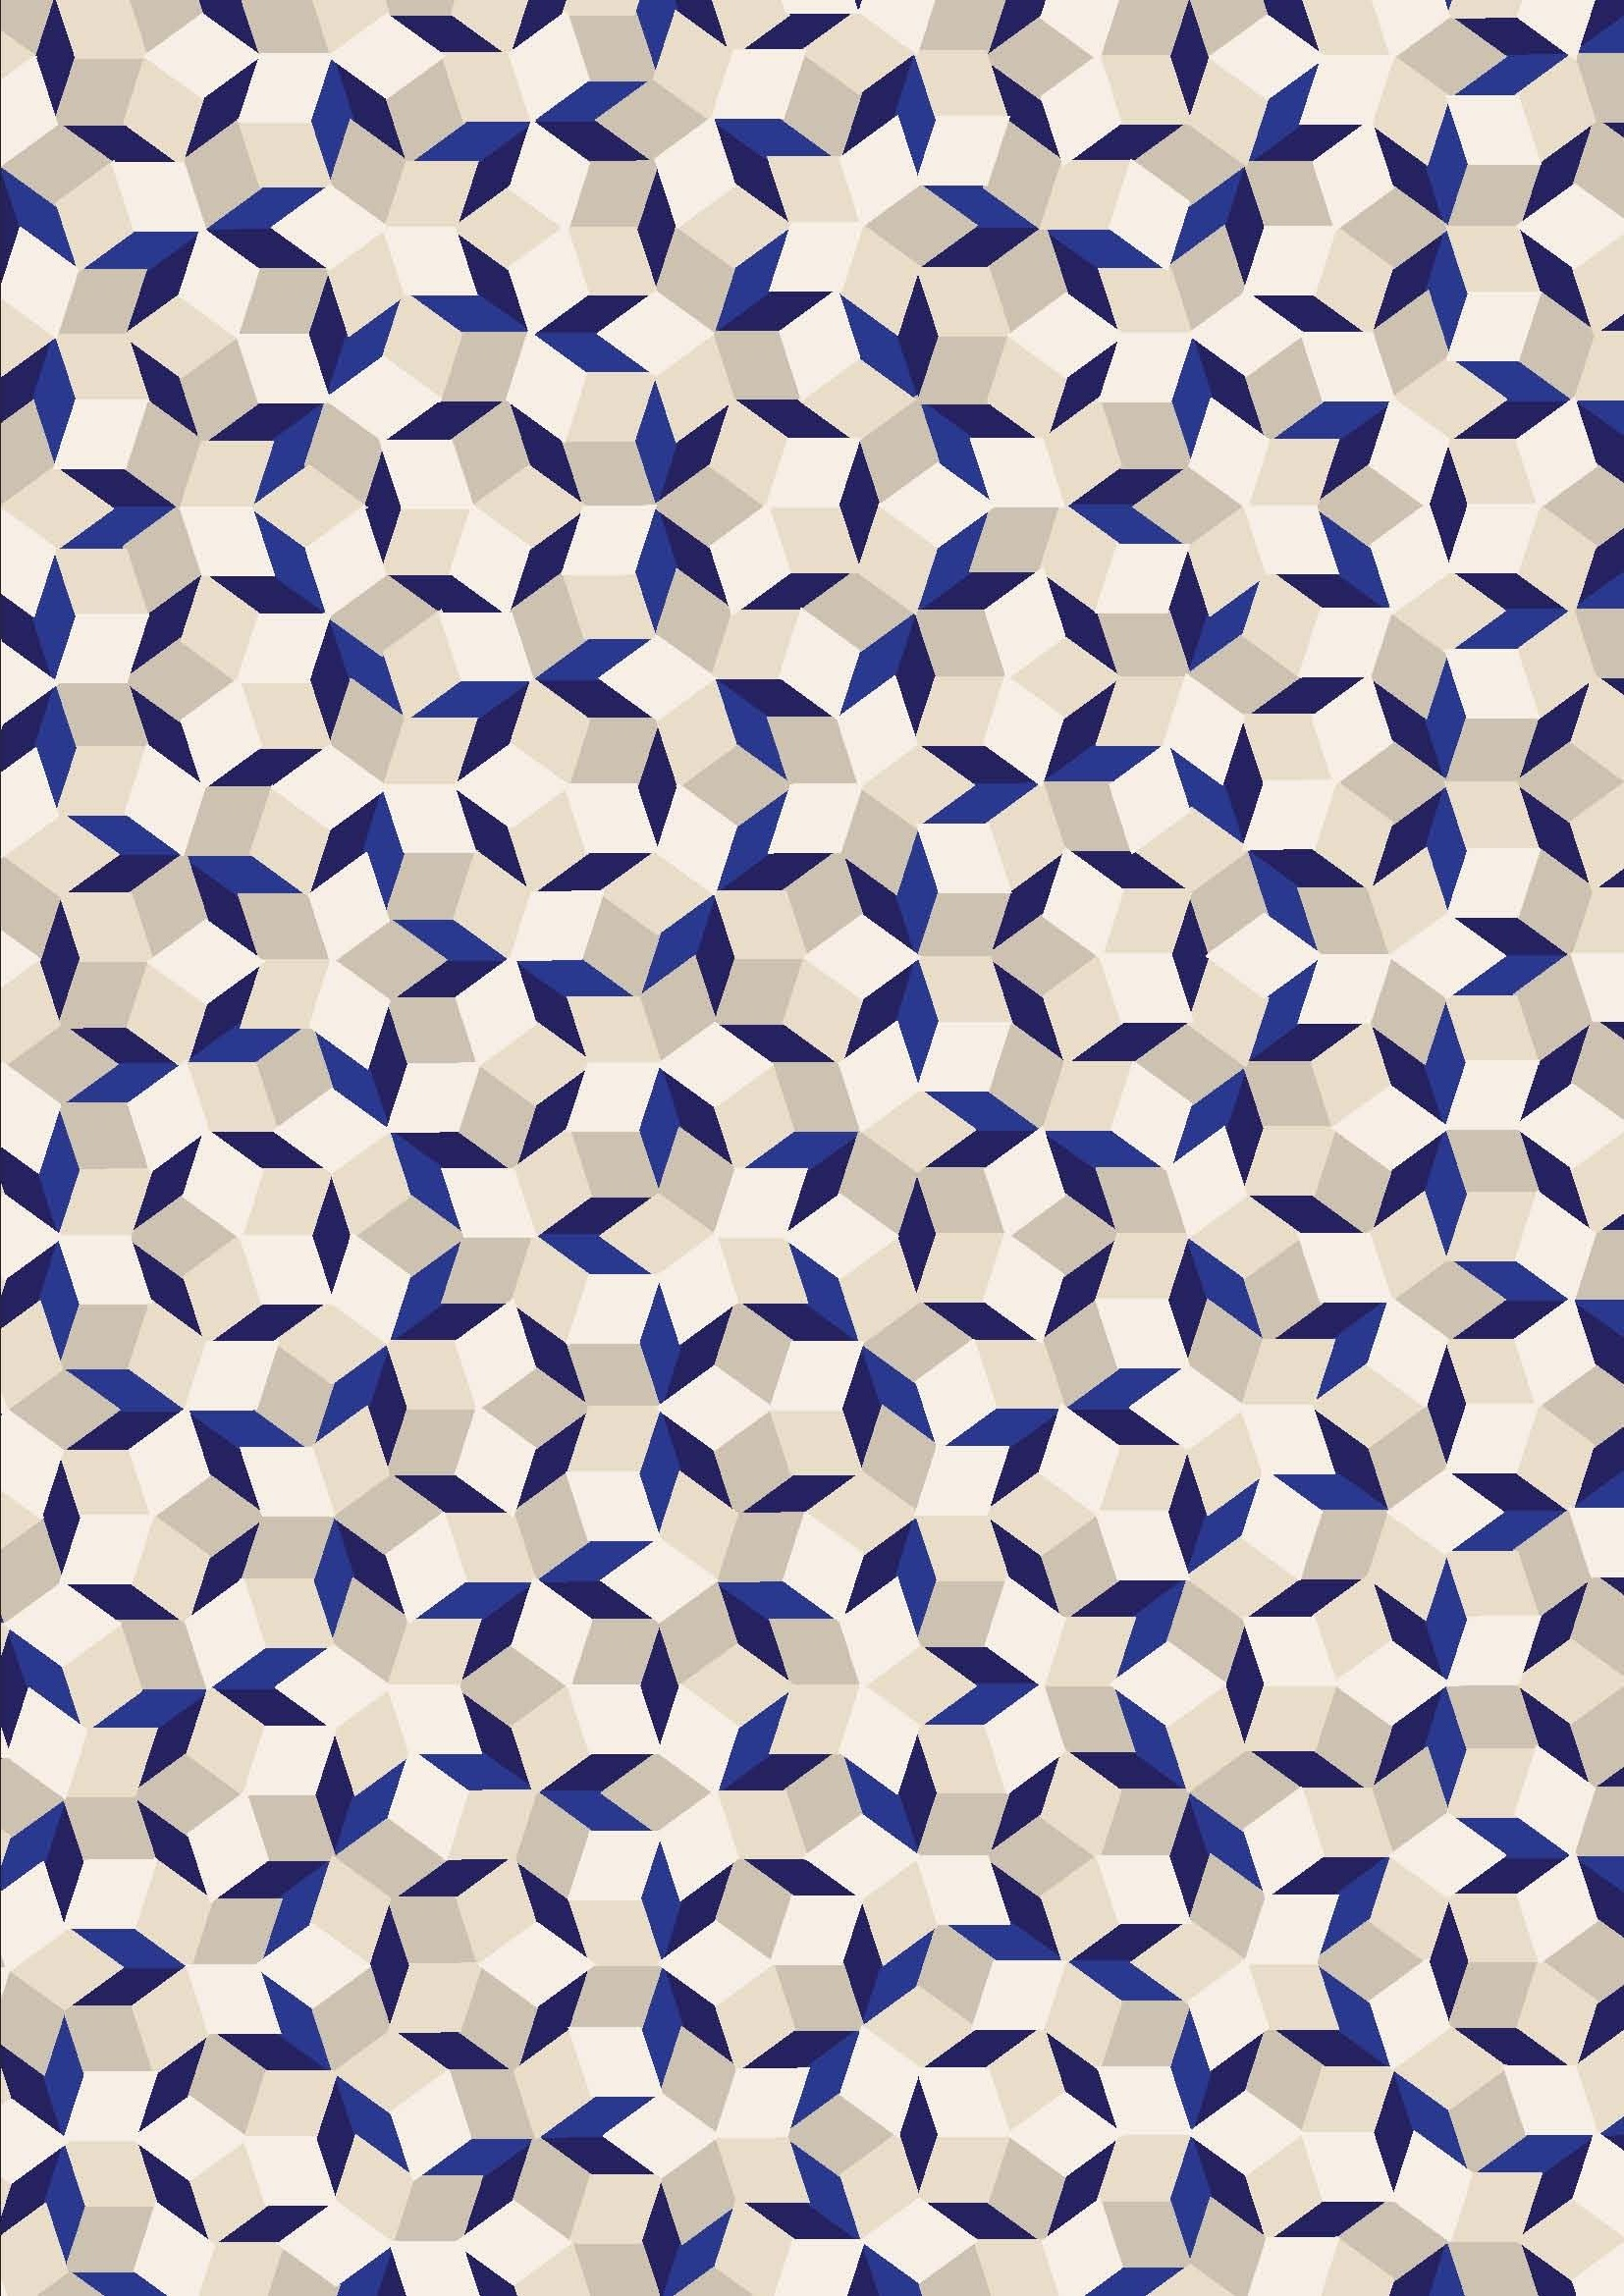
\includegraphics[width=\paperwidth,height=\paperheight]{images/penrose2r.jpg}}%
}

\newcommand\numberthis{\addtocounter{equation}{1}\tag{\theequation}}

\newtcolorbox{MyOuterBox}{%
  enhanced,
  % watermark graphics=images/santa_faces_watermark.jpg,
  % watermark opacity=0.8,
  % watermark zoom=2.0,
  breakable,
  frame style=JISpurple,
  colback=JISivory,
  colframe=JISpurple,
  title={
\includegraphics[width=0.9cm,height=0.9cm]{images/JIS Final Logo FA-02.png}\raisebox{3mm}{\Large{Maths Challenge}\hspace{24em} \Large{\bfseries\sffamily 17}}},
}

\newtcolorbox{MyInnerBox}[2][]{enhanced,%empty,
coltitle=JISpurple,colback=white,
breakable,
fonttitle=\bfseries\sffamily,
attach boxed title to top left={yshift=-1.5mm},
boxed title style={empty, size=small, top=1mm, bottom=0pt},
varwidth boxed title=0.5\linewidth,
frame code={
  \path (title.east|-frame.north) coordinate (aux);
\path[draw=JISpurple, line width=0.5mm, rounded corners,fill=white]
(frame.west) |- ([xshift=-2.5mm]title.north east) to[out=0, in=180] ([xshift=7.5mm]aux)-|(frame.east)|-(frame.south)-|cycle;
},
title={#2},#1}

\newtcolorbox{MyInnerSplitBox}[2][]{enhanced,%empty,
bicolor,sidebyside,sidebyside align=top seam,
righthand width=7.5cm,colbacklower=white,
sidebyside gap=5mm,
breakable,
coltitle=JISpurple,colback=white,
fonttitle=\bfseries\sffamily,
attach boxed title to top left={yshift=-1.5mm},
boxed title style={empty, size=small, top=1mm, bottom=0pt},
varwidth boxed title=0.5\linewidth,
frame code={
  \path (title.east|-frame.north) coordinate (aux);
\path[draw=JISpurple, line width=0.5mm, rounded corners,fill=white]
(frame.west) |- ([xshift=-2.5mm]title.north east) to[out=0, in=180] ([xshift=7.5mm]aux)-|(frame.east)|-(frame.south)-|cycle;
},
title={#2},#1}


\newtcolorbox{MySolutionBox}[1][]{%
  enhanced,
  breakable,
  frame style=JISpurple,
  colback=PaleGreen, colframe=green,
  title={\Large Solution},
  drop fuzzy shadow,
  halign=left,
  #1
}

%%%%%%%%%%%%%%%%%%%%%%%%%%%%%%%%%%%%%%%%%%%%%%%%%%
\newtoggle{SOLUTION}
%%% Uncomment the appropriate line below to show solutions %%%
% \toggletrue{SOLUTION}
\togglefalse{SOLUTION}
%%%%%%%%%%%%%%%%%%%%%%%%%%%%%%%%%%%%%%%%%%%%%%%%%


%%%%%%%%%%%%%%%%%%%%%%%%%%%%%%%%%%%%%%%%%%%%%%%%%%
%%%%%%            DOCUMENT BEGINS           %%%%%%
%%%%%%%%%%%%%%%%%%%%%%%%%%%%%%%%%%%%%%%%%%%%%%%%%%
\begin{document}


  \begin{MyOuterBox}
    \iftoggle{SOLUTION}{Here are the full, or partial solutions.
    }{
      Welcome to this week's Maths Challenge!\\
      Have a go at both questions!\\
      Drop your solution in the box in the staffroom by Tuesday.
    }
       \begin{MyInnerBox}{Year 8 and below}
     In Shakespeare's 'Merchant of Venice', Portia had three caskets - lead, silver and gold - inside one of which was Portia's portrait. Raymond Smullyan used this idea to write a series of logic puzzles, two of which you see here. To win the prize (one minute in the Total Perspective Vortex) you must say which casket holds the portrait. Portia tells you that, of the three statements on the caskets, at most one is true. Portia is truthful.\par\vspace{3mm}
        \begin{tikzpicture}[scale=0.8,font=\fontfamily{TrajanP}\selectfont]
          \path[draw,line width=3mm,DarkGoldenrod1,fill overzoom image=images/wp7316403.jpg] (1,1.5) to[bend left=45] (1.5,1) -- (6.5,1) to[bend left=45] (7,1.5) -- (7,4.5) to[bend left=45] (6.5,5)-- (1.5,5) to[bend left=45] (1,4.5) -- cycle;
          \path[draw,line width=0.5mm,DarkGoldenrod4] (1.4,1.9) to[bend left=45] (1.9,1.4) -- (6.1,1.4) to[bend left=45] (6.6,1.9) -- (6.6,4.1) to[bend left=45] (6.1,4.6)-- (1.9,4.6) to[bend left=45] (1.4,4.1) -- cycle;
          \path[fill overzoom image=images/goldbrush.jpg] (2.0,2.0) -- (6.0,2.0) -- (6.0,4.0) -- (2.0,4.0) -- cycle;
          \node[black,align=center,text width=4cm] at (4,3.0) {\baselineskip=20pt\TrajanP The \textbf{Portrait} is\\\TrajanP in this casket\par};
        \end{tikzpicture}\hspace{2mm}
        \begin{tikzpicture}[scale=0.8]
          \path[draw,line width=3mm,Snow2,fill overzoom image=images/SilverFoil.jpg] (1,1.5) to[bend left=45] (1.5,1) -- (6.5,1) to[bend left=45] (7,1.5) -- (7,4.5) to[bend left=45] (6.5,5)-- (1.5,5) to[bend left=45] (1,4.5) -- cycle;
          \path[draw,line width=0.5mm,white] (1.4,1.9) to[bend left=45] (1.9,1.4) -- (6.1,1.4) to[bend left=45] (6.6,1.9) -- (6.6,4.1) to[bend left=45] (6.1,4.6)-- (1.9,4.6) to[bend left=45] (1.4,4.1) -- cycle;
          \path[fill overzoom image=images/silverBg.jpg] (2.0,2.0) -- (6.0,2.0) -- (6.0,4.0) -- (2.0,4.0) -- cycle;
          \node[black,align=center,text width=4cm] at (4,3.0) {\baselineskip=15pt\TrajanP The \textbf{Portrait} is\\\TrajanP not in\\\TrajanP this casket\par};
        \end{tikzpicture}\hspace{2mm}
        \begin{tikzpicture}[scale=0.8]
          \path[draw,line width=3mm,SlateGray4,fill overzoom image=images/LeadBg.jpg] (1,1.5) to[bend left=45] (1.5,1) -- (6.5,1) to[bend left=45] (7,1.5) -- (7,4.5) to[bend left=45] (6.5,5)-- (1.5,5) to[bend left=45] (1,4.5) -- cycle;
          \path[draw,line width=0.5mm,black] (1.4,1.9) to[bend left=45] (1.9,1.4) -- (6.1,1.4) to[bend left=45] (6.6,1.9) -- (6.6,4.1) to[bend left=45] (6.1,4.6)-- (1.9,4.6) to[bend left=45] (1.4,4.1) -- cycle;
          \path[fill=Ivory3,opacity=0.3] (2.0,2.0) -- (6.0,2.0) -- (6.0,4.0) -- (2.0,4.0) -- cycle;
          \node[black,align=center,text width=4cm] at (4,3.0) {\baselineskip=15pt\TrajanP The \textbf{Portrait} is\\\TrajanP not in the\\\TrajanP gold casket\par};
        \end{tikzpicture}
      \iftoggle{SOLUTION}{%conditional output begin
      \begin{MySolutionBox}
        We start off with the assumption that the question is correct, Portia is truthful, and therefore, it is true that exactly one of the statements is true, or, they are all false.\par
        We then proceed by cases: we look at each possibility in turn. We eliminate the possibilities that give rise to impossible situations.\par
        \underline{Case 1: All statements are false}\par
        \hspace{1em}Gold: \;The statement on this casket is false: the portrait is not in the gold casket.\par
        \hspace{1em}Silver: The statement is false: the portrait is in this casket.\par
        \hspace{1em}Lead: \;The statement is false: the portrait is in the gold casket.\par
        We have an inconsistency, this line of reasoning tells us the portrait is in two caskets at the same time, so we reject Case 1.\par\medskip
        \underline{Case 2: The statement on the gold casket is true}\par
        \hspace{1em}Gold: \;The statement is true: the portrait is in the gold casket.\par
        \hspace{1em}Silver: The statement is false: the portrait is in the silver casket.\par
        \hspace{1em}Lead: \;The statement is false: the portrait is in gold casket.\par
        Again we have an inconsistency, we have found the portrait is in the silver and gold caskets at the same time, so we reject Case 1.\par\medskip
        \underline{Case 3: The statement on the silver casket is true}\par
        \hspace{1em}Gold: \;The statement is false: the portrait is not in the gold casket.\par
        \hspace{1em}Silver: The statement is true: the portrait is not in the silver casket.\par
        \hspace{1em}Lead: \;The statement is false: the portrait is in the gold casket.\par
        Once again, our assumption has led to a contradiction, here the portrait is simultaneously in, and not in, the gold casket.\par\medskip
        \underline{Case 4: The statement on the lead casket is true}\par
        \hspace{1em}Gold: \;The statement is false: the portrait is not in the gold casket.\par
        \hspace{1em}Silver: The statement is false: the portrait is in the silver casket.\par
        \hspace{1em}Lead: \;The statement is true: the portrait is not in the gold casket.\par
        This time, we did not arrive at a logical impossibility, so, the portrait is in the silver casket.\par\medskip
        We have looked at a methodical path to our solution. We could also have noticed that the statements on the gold casket and the lead casket say the opposite, so one of them must be true. Since at most, one of the statements is true, the statement on the silver casket must be false. Therefore the portrait is in the silver casket.\par
      \end{MySolutionBox}
    }{}%conditional output end
    \end{MyInnerBox}


    \vspace{0.4cm}
          \begin{MyInnerBox}{Year 9 and above}
        Please read the introduction above, and try the first puzzle.\par
        This time Portia explains to you that at least one of the three statements is true and that at least one of the three statements is false. Portia is truthful. Which casket holds the portrait?\par\vspace{3mm}
        \begin{tikzpicture}[scale=0.8,font=\fontfamily{TrajanP}\selectfont]
          \path[draw,line width=3mm,DarkGoldenrod1,fill overzoom image=images/wp7316403.jpg] (1,1.5) to[bend left=45] (1.5,1) -- (6.5,1) to[bend left=45] (7,1.5) -- (7,4.5) to[bend left=45] (6.5,5)-- (1.5,5) to[bend left=45] (1,4.5) -- cycle;
          \path[draw,line width=0.5mm,DarkGoldenrod4] (1.4,1.9) to[bend left=45] (1.9,1.4) -- (6.1,1.4) to[bend left=45] (6.6,1.9) -- (6.6,4.1) to[bend left=45] (6.1,4.6)-- (1.9,4.6) to[bend left=45] (1.4,4.1) -- cycle;
          \path[fill overzoom image=images/goldbrush.jpg] (2.0,2.0) -- (6.0,2.0) -- (6.0,4.0) -- (2.0,4.0) -- cycle;
          \node[black,align=center,text width=4cm] at (4,3.0) {\baselineskip=15pt\TrajanP The \textbf{Portrait} is\\\TrajanP not in the\\\TrajanP silver casket\par};
        \end{tikzpicture}\hspace{2mm}
        \begin{tikzpicture}[scale=0.8]
          \path[draw,line width=3mm,Snow2,fill overzoom image=images/SilverFoil.jpg] (1,1.5) to[bend left=45] (1.5,1) -- (6.5,1) to[bend left=45] (7,1.5) -- (7,4.5) to[bend left=45] (6.5,5)-- (1.5,5) to[bend left=45] (1,4.5) -- cycle;
          \path[draw,line width=0.5mm,white] (1.4,1.9) to[bend left=45] (1.9,1.4) -- (6.1,1.4) to[bend left=45] (6.6,1.9) -- (6.6,4.1) to[bend left=45] (6.1,4.6)-- (1.9,4.6) to[bend left=45] (1.4,4.1) -- cycle;
          \path[fill overzoom image=images/silverBg.jpg] (2.0,2.0) -- (6.0,2.0) -- (6.0,4.0) -- (2.0,4.0) -- cycle;
          \node[black,align=center,text width=4cm] at (4,3.0) {\baselineskip=15pt\TrajanP The \textbf{Portrait} is\\\TrajanP not in\\\TrajanP this casket\par};
        \end{tikzpicture}\hspace{2mm}
        \begin{tikzpicture}[scale=0.8]
          \path[draw,line width=3mm,SlateGray4,fill overzoom image=images/LeadBg.jpg] (1,1.5) to[bend left=45] (1.5,1) -- (6.5,1) to[bend left=45] (7,1.5) -- (7,4.5) to[bend left=45] (6.5,5)-- (1.5,5) to[bend left=45] (1,4.5) -- cycle;
          \path[draw,line width=0.5mm,black] (1.4,1.9) to[bend left=45] (1.9,1.4) -- (6.1,1.4) to[bend left=45] (6.6,1.9) -- (6.6,4.1) to[bend left=45] (6.1,4.6)-- (1.9,4.6) to[bend left=45] (1.4,4.1) -- cycle;
          \path[fill=Ivory3,opacity=0.3] (2.0,2.0) -- (6.0,2.0) -- (6.0,4.0) -- (2.0,4.0) -- cycle;
          \node[black,align=center,text width=4cm] at (4,3.0) {\baselineskip=15pt\TrajanP The \textbf{Portrait} is\\\TrajanP in this casket\par};
        \end{tikzpicture}
      \iftoggle{SOLUTION}{%conditional output begin
      \begin{MySolutionBox}
        We could proceed by cases - taking each statement as true in turn - as in the solution to the first puzzle. To illustrate a different approach, we are going to proceed by cases but assume the portrait is in each casket in turn, and see what that leads to.\par
        \underline{Case 1: The portrait is in the gold casket}\par
        \hspace{1em}The gold and silver statements are true. The lead statement is false. No inconsistencies, but let's check the other two cases anyway.\par\medskip
        \underline{Case 2: The portrait is in the silver casket}\par
        \hspace{1em}The gold, silver and lead statements are all false, but this contradicts what Portia told you, that at least one statement must be true.\par\medskip
        \underline{Case 3: The portrait is in the lead casket}\par
        \hspace{1em}The gold, silver and lead statements are all true, again, this contradicts what Portia told you.\par\medskip
        So the first case is correct, the portrait is in the gold casket.\par
      \end{MySolutionBox}
    }{}%conditional output end
    \end{MyInnerBox}


  \end{MyOuterBox}

%%%%%%%%%%%%%%%%%%%%%%%%%%%%%%%%%%%%%%%%%%%%%%%%%%
\end{document}



